\documentclass{article}

\usepackage{graphicx}
\usepackage{booktabs} 
\usepackage[section]{placeins}

\begin{document}

\section{Didge Report No 0}

\subsection{Shape}
\begin{centering}
\begin{tabular}{ll}
\toprule
          length &  1697.951382 \\
       bell size &    98.310392 \\
 number segments &           33 \\
     tuning\_loss &         1.48 \\
     volume\_loss &         0.68 \\
     n\_note\_loss &         0.00 \\
   diameter\_loss &         0.05 \\
fundamental\_loss &         0.14 \\
     octave\_loss &         0.16 \\
            loss &         2.52 \\
\bottomrule
\end{tabular}
\end{centering}


\begin{centering}
\begin{figure}[!h]
{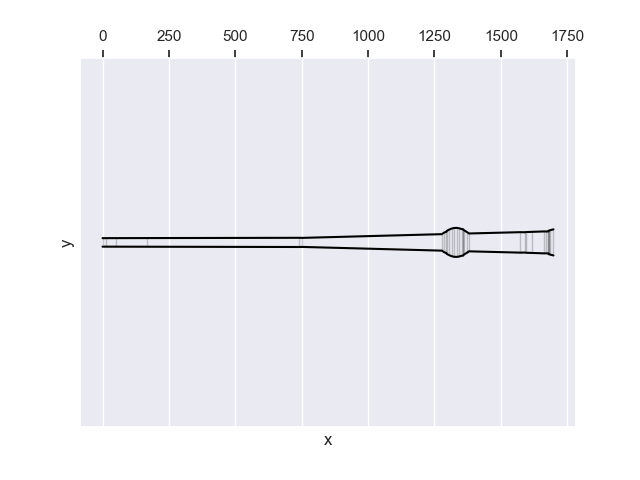
\includegraphics[width=\textwidth]
{0_didge.png}}
\caption{Didge 1}
\end{figure}
\end{centering}

\subsection{Tuning}
\begin{centering}
\begin{tabular}{rrrrrl}
\toprule
 freq &    impedance &  rel\_imp &  note-number &  cent-diff & note-name \\
\midrule
 73.4 & 2.822999e+07 & 1.000000 &          -31 &   0.381867 &        D1 \\
147.0 & 5.416363e+06 & 0.191866 &          -19 &  -1.975158 &        D2 \\
247.0 & 6.670754e+06 & 0.236300 &          -10 &  -0.409022 &        B3 \\
348.0 & 5.385137e+06 & 0.190759 &           -4 &   6.099461 &        F3 \\
994.0 & 3.490873e+06 & 0.123658 &           14 & -10.890794 &        B5 \\
\bottomrule
\end{tabular}
\end{centering}
\subsection{Evolution Parameters}

cad.calc.parameters.AddPointOptimizer

\begin{centering}
\begin{tabular}{lllll}
\toprule
name & value &  min &  max &  mutable \\
\midrule
  x0 &  0.80 & 0.00 & 1.00 &    False \\
  y0 &  1.01 & 0.50 & 1.50 &    False \\
\bottomrule
\end{tabular}
\end{centering}
\subsection{Sound Spektra}

    \begin{figure}[!h]
    {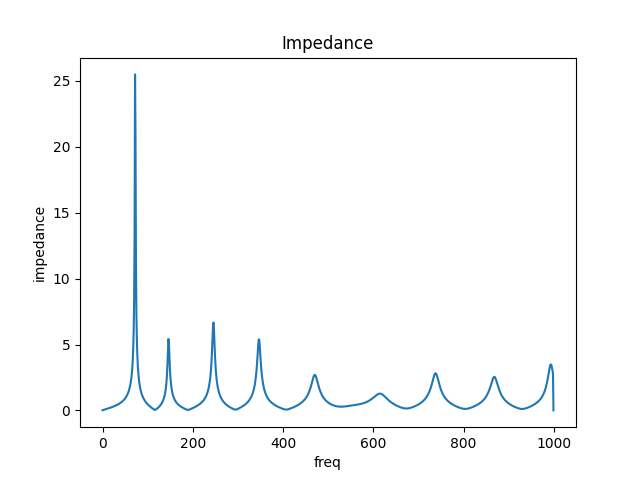
\includegraphics[width=100mm]
    {0_impedance.png}
    \caption{Impedance Spektrum 1}}
    \end{figure}
    \begin{figure}[!h]
        \begin{tabular}{cc}
                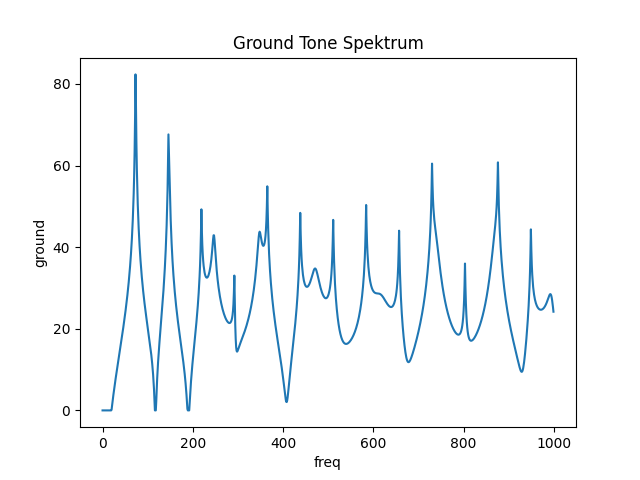
\includegraphics[width=75mm]{0_ground.png} &  
                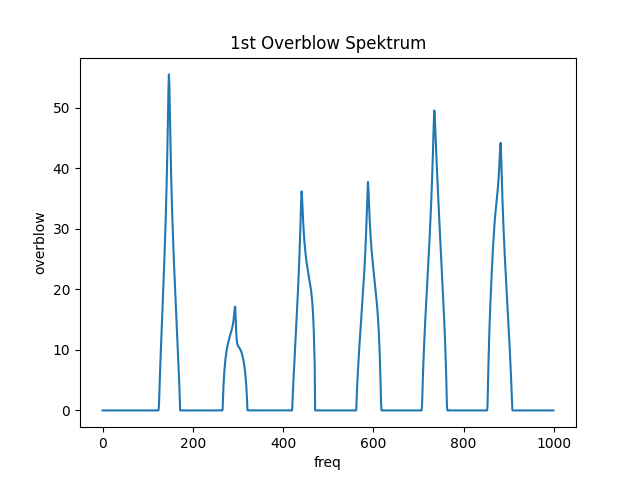
\includegraphics[width=75mm]{0_overblow} \\
        \end{tabular}
    \caption{Spektra 1}
    \end{figure}
    \end{document}